\chapter{Dataanalyse}
Denne fasen, og den foregående, er de vi har fokusert mest på i prosessen. Hvis en av de gjøres ufullstendig vil det være kritisk for resultatet av oppgaven. I denne fasen analyseres dataene som er samlet inn, og ved hjelp av statistiske verktøy kan vi trekke konklusjoner basert på svarene. Under dataanalysen kommer vi til å bruke generelle statistiske verktøy for å illustrere svarene og sammenhengene mellom de. Hovedfokuset i denne fasen er likevel å fokusere på de verktøyene som er beskrevet i boken om rotårsaksanalyse \cite{RCA}, men vi utelukker ikke bruk av annet vi anser som nyttig. Etter denne fasen ønsker vi å sitte igjen med mulige årsaker til at folk driver med ulovlig fildeling, samt andre relevante data relatert til fildeling. Verktøyet vi har brukt til å gjøre mesteparten av analysene er SPSS, et statistisk verktøy for å blant annet gjøre grafiske- og matematiske beregninger.

\section{Demografi}
I spørreundersøkelsen ble informasjon om fire forskjellige demografier samlet inn: Kjønn, fakultet, studentby og alder. Det er viktig å nevnte at det ikke ble samlet inn lik mengde svar fra alle kategoriene, så dette må vi tenke på når vi analyserer dataene. Det var for eksempel overvekt av menn som besvarte undersøkelsen. Av respondentene var det 27.8\% kvinner og 72.2\%. Det var også overvekt av personer som er mellom 20 og 25 år, disse tilsvarte 74.2\% av de spurte. På fakultet og studentby ønsket vi i hovedsak å få inn relativt spredte svar, men det ble overvekt av personer fra fakultet for informasjonsteknologi og elektroteknikk, og også en overvekt av personer fra Kallerud studentby. Disse inkluderte henholdsvis 50.5\% og 52\% av respondentene. De komplette frekvenstabellene over demografien finnes i \hyperref[frekvens]{Vedlegg C}.

\section{Analyse ved hjelp av histogram}
Histogrammer brukes til å vise distribusjonen og variasjonen i et spesifikt datasett. Hovedgrunnen til å bruke histogrammer er for å skape en visuell forståelse av dataene som en ellers ikke får fra tabeller o.l. Da blir det enklere å se korrelasjoner og sammenhenger i datasettet. Innen rotårsaksanalyse brukes det ofte for å visualisere hvilke mulige rotårsaker som er mest utbredt, og forstå distribusjonen av hendelser, problemer, årsaker, konsekvenser osv. \cite{RCA}

\subsection{Ønsket utbytte}
Ønsket utbytte ved bruk av histogrammer er en visualisering av de mest utbredte mulige rotårsakene, samt info om andre relevante aspekter ved oppgaven. Analyse av spørsmålene tilknyttet likert-skala er viktig for å finne mulige rotårsaker. Ellers ønsker vi også å finne sammenhenger mellom de ulike spørsmålene, for å se relevante korrelasjoner mellom de.


\subsection{Gjennomføring og resultater}
Vi starten analysen ved å undersøke hvor mange som faktisk laster ned av de spurte. Dette ble gjort i SPSS og arrangert etter prosentandel. Resultatet konkluderte med at det er 35\% som har lastet ned og 65\% som ikke har gjort det, som vist i histogrammet under.

\begin{figure}[H]
    \centering
    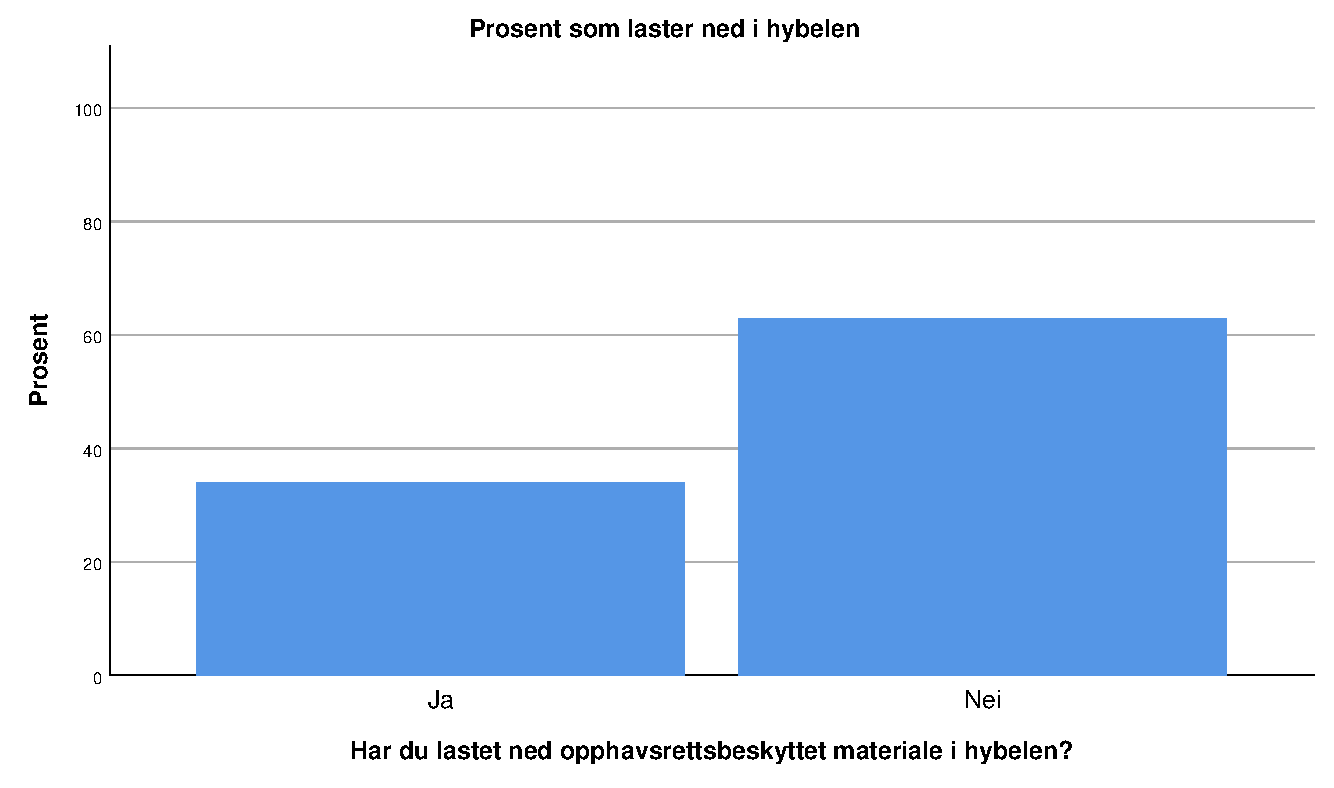
\includegraphics[scale=0.45]{case_1/bilder/lasterned.pdf}
    \label{fig:lasterned}
    \caption[Laster ned]{Hvor mange som laster ned av de spurte}
\end{figure}

Vi kan se på histogrammet at flertallet ikke laster ned, som var noe flere enn vi forventet, men det er fortsatt en stor andel som faktisk laster ned ulovlig. Det har også en liten innvirkning at en stor andel av respondentene kom fra informatikk- og datarelaterte studier, så vi kan fastslå at gjennomsnittet egentlig ligger noe lavere på nedlasting, men ikke med mye. Dette vises i \hyperref[fig:IT-lasterned]{følgende histogram}.

\subsubsection{Kjønnsforskjeller}
Vi ønsket også å undersøke om det er noen forskjeller i hvem som laster ned basert på kjønn. Under ser vi forholdet mellom kjønnene.
\begin{figure}[H]
    \centering
    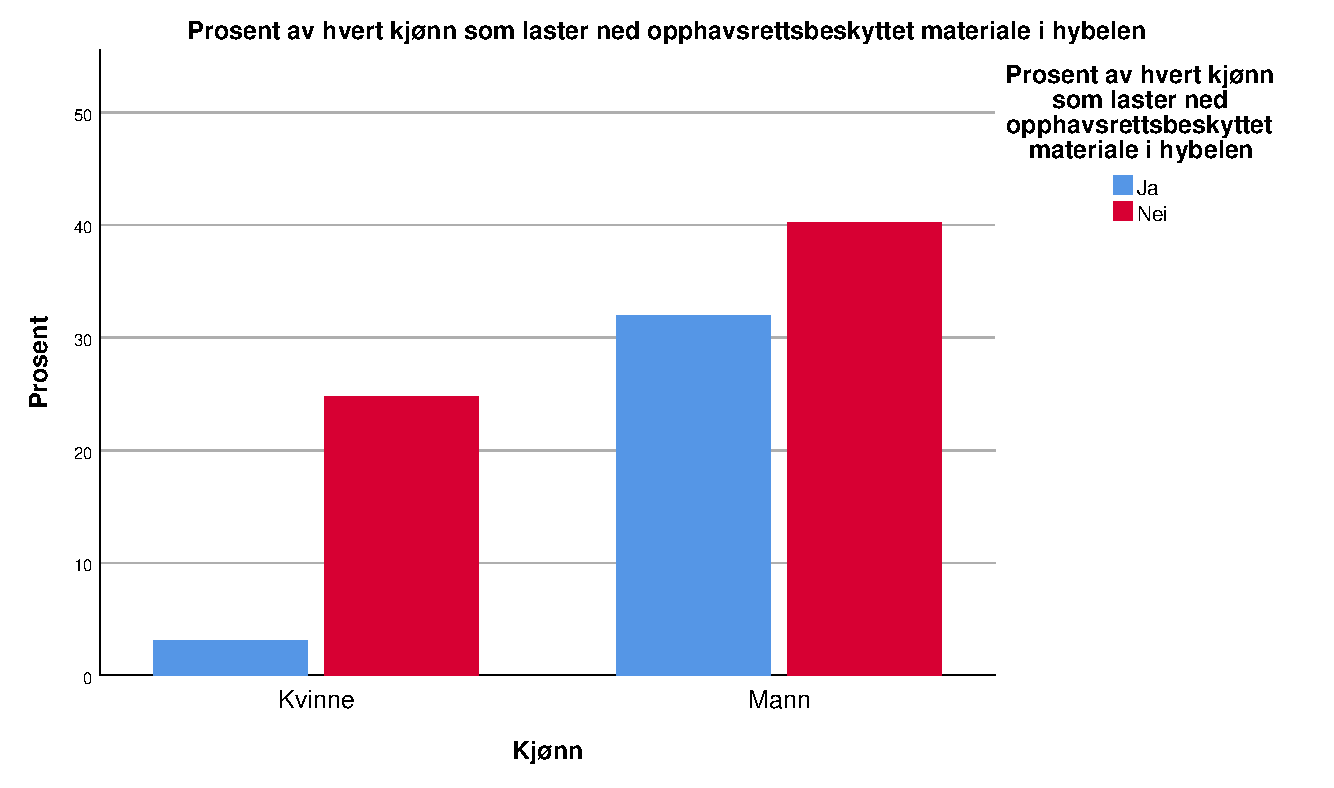
\includegraphics[scale=0.45]{case_1/bilder/kjonn_lasterned.pdf}
    \label{fig:kjønn_lasterned}
    \caption[Kjønn laster ned]{Hvor mange fra hvert kjønn som laster ned}
\end{figure}
Vi kan se over at det er i hovedsak menn som laster ned ulovlig, mens kvinner har svart at de i stor grad ikke laster ned. Dette blir selvfølgelig påvirket at det er få kvinner i IT-relaterte studier, som vi har funnet ut at utgjør noe mer av nedlastingen. Det er derimot vanskelig å vite helt sikkert om det er fordi kvinner er underrepresentert i IT studier som gir utslag, eller om det er kvinner generelt sett som ikke laster ned. Der er likevel en mer signifikant forskjell mellom kjønnene enn det er mellom IT studier og andre studier som vist i figur \ref{fig:IT-lasterned}, så vi velger å tolke det som at kvinner laster ned mindre enn menn.

\subsubsection{Forskjeller mellom studentbyer}
Samtlige studentbyer har et kablet nettverk av Uninett godt egnet for nedlasting, enten det er lovlig eller ulovlig nedlasting. Det er derimot noen forskjeller i hastighet på enkelte studentbyer. Nordbyen, Sørbyen og Sentrum har muligheten til 100Mbps nedlasting og 100Mbps opplasting, mens Kallerud har en øvre grense på hele 1000Mbps nedlasting og 1000Mbps opplasting. Dette er ti ganger hastigheten til de andre studentbyene. Derfor ønsket vi å undersøke om dette hadde noe relevans i forhold til hvor mange som laster ned ulovlig. 

\begin{figure}[H]
    \centering
    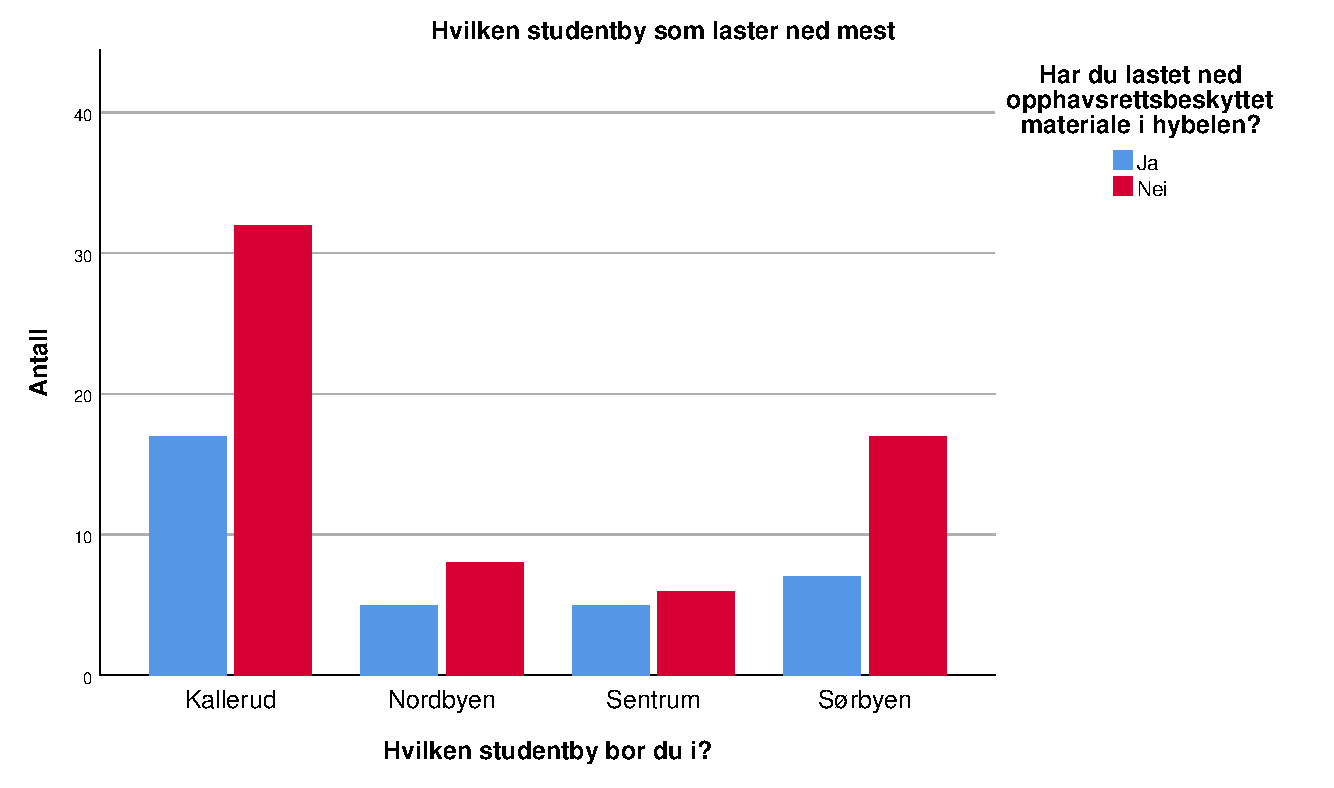
\includegraphics[scale=0.45]{case_1/bilder/studentby_lasterned.pdf}
    \label{fig:studentby_lasterned}
    \caption[Studentby laster ned]{Hvor mange fra hver studentby som laster ned}
\end{figure}

På grunn av lav oppslutning på Nordbyen og Sentrum er det vanskelig å si noe sikkert på dem, mens Kallerud og Sørbyen ikke varierer så veldig fra hverandre. Når vi bruker histogrammer ser vi ingen signifikant forskjell mellom studentbyene når det kommer til nedlasting som vi kan si med sikkerhet.

\subsubsection{Konsekvenser ved nedlasting}
Et spørsmål som ble spurt i spørreundersøkelsen var hvor godt kjent de var med mulige konsekvenser ved ulovlig nedlasting, og med det brudd på opphavsretten. Det kunne være relevant å se om det var noen spesiell sammenheng mellom de som ikke kjente til konsekvensene og de som lastet ned. 

\begin{figure}[H]
    \centering
    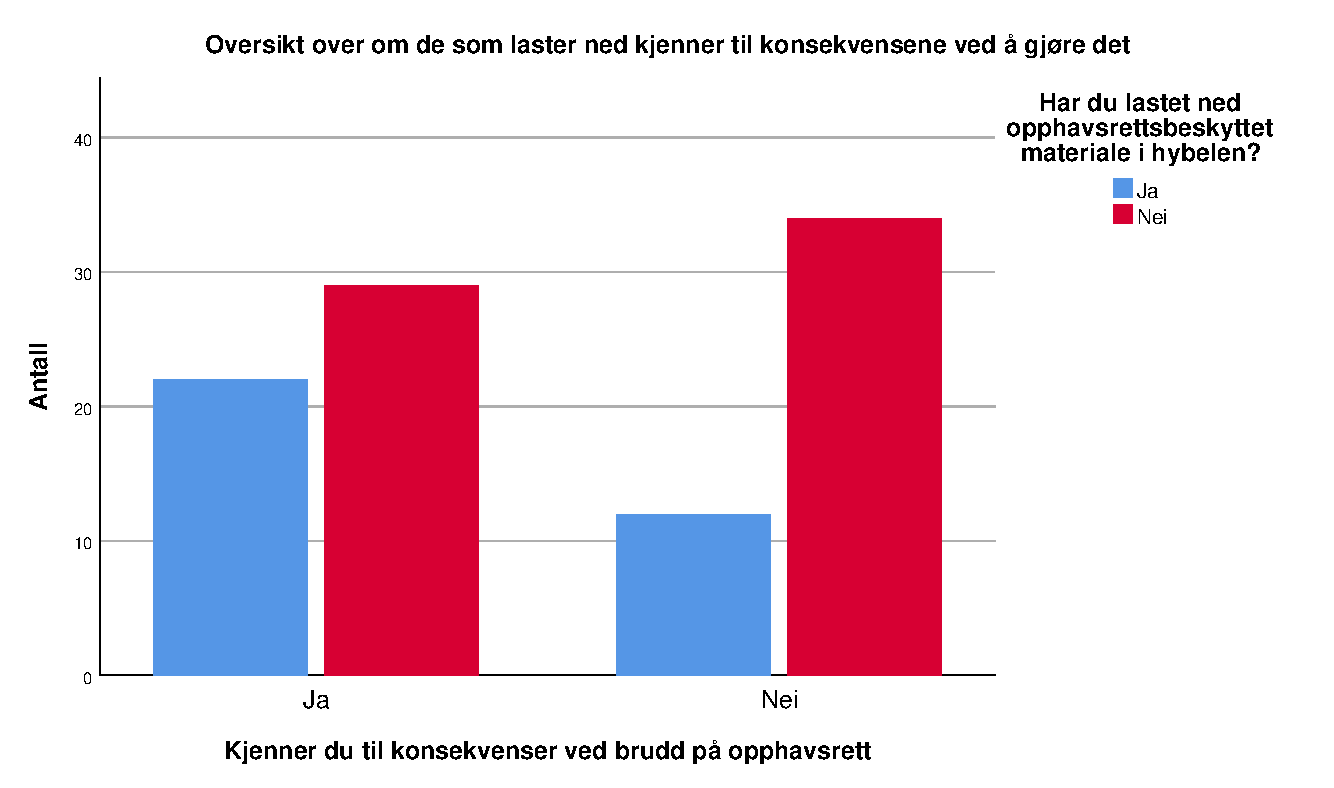
\includegraphics[scale=0.45]{case_1/bilder/konsekvens_lasterned.pdf}
    \label{fig:konsekvens_lasterned}
    \caption[Konsekvens av å laste ned]{Hvor mange som kjenner til konsekvenser ved å laste ned}
\end{figure}

Det viser seg faktisk at de som laster ned har bedre kjennskap til konsekvensene enn de som ikke gjør det. Det kan kanskje ha noe å gjøre med at de er mer opptatt av problemområdet enn de som ikke laster ned. De som ikke laster ned i første omgang har kanskje ingen grunn til å sjekke konsekvensene av det. I tillegg fant vi ut at IT-studenter kjenner konsekvenser bedre enn de andre, og de har også høyere andel nedlastere. Vi prøvde å kjøre samme test på hvor godt de kjenner til IT-reglementet til NTNU \cite{ITReg} og kom til samme konklusjon som over. Dette histogrammet kan sees \hyperref[fig:reglement-lasterned]{her}. En grunn til dette er også igjen at IT-studenter kjenner bedre til IT reglementet, som vist \hyperref[fig:reglement-fakultet]{her}, og de er i overvekt. Så dette må tas i betraktning. 

En mulig teori vi ønsket å prøve ut var om mange som lastet ned ikke kjente til konsekvensene ved ulovlig nedlasting eller NTNU sitt IT-reglementet, og lastet ned på grunn av det. Dette ble altså delvis motbevist.

\subsubsection{Årsaker til nedlasting}
I spørreundersøkelsen kom vi med seks påstander til hvorfor respondentene laster ned, som de besvarte på en likert-skala fra 1 til 5, der 1 er i liten grad og 5 er i stor grad. Etter å ha analysert alle seks påstandene ved hjelp av SPSS og histogrammer fant vi én påstand som hadde en graftopp der respondentene svarte positivt. De aller fleste svarte de var enige i at de lastet ned på grunn av tilgjengelighet.

\begin{figure}[H]
    \centering
    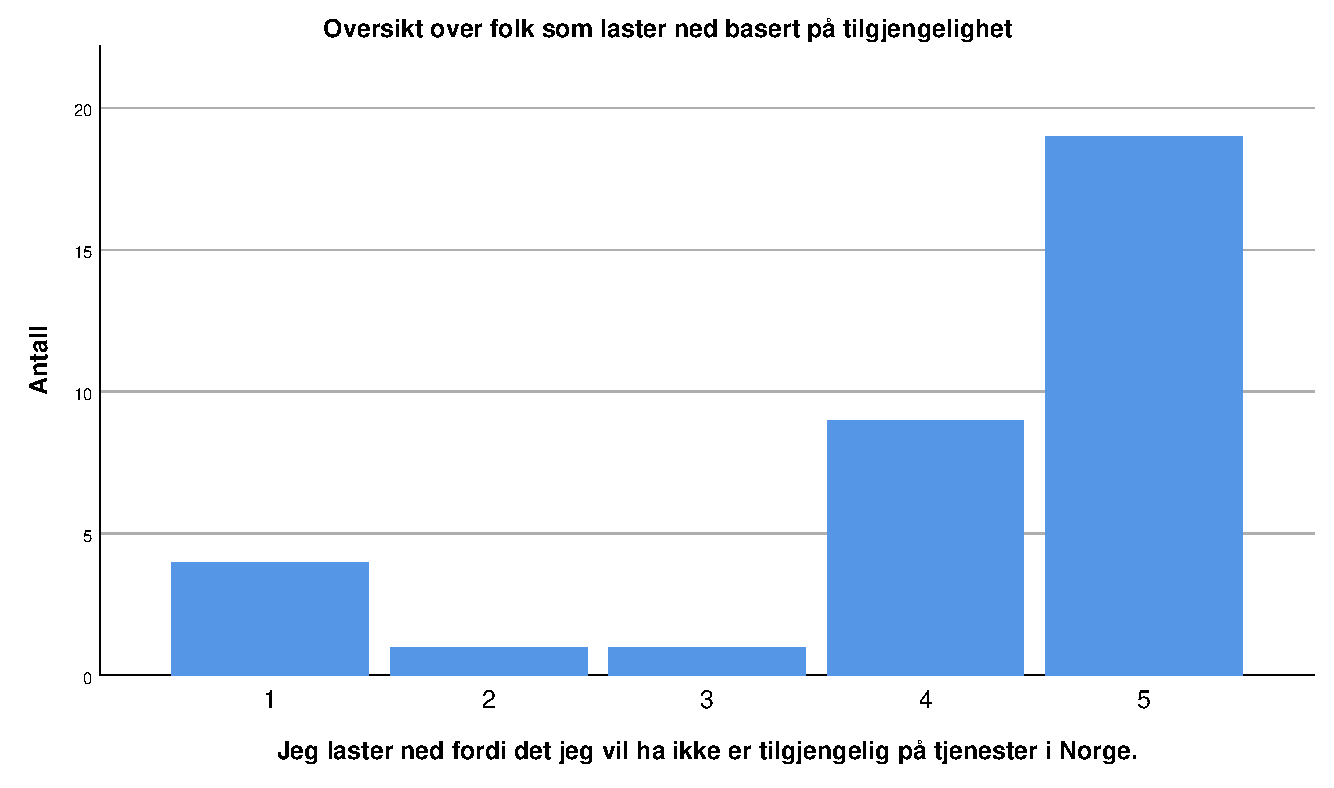
\includegraphics[scale=0.45]{case_1/bilder/tilgjengelighet.pdf}
    \label{fig:tilgjengelighet}
    \caption[Tilgjengelighet]{Hvor mange som laster ned av de spurte}
\end{figure}

Dette vil si at det er godt mulig at tilgjengeligheten er en årsak til om en laster ned eller ikke, og er verdt å dokumentere til videre analyse. Siden tilgjengelighet betyr så mye, var det naturlig å utforske det ytterligere. Vi fant ut at det kunne være relevant å vite om de som brydde seg om tilgjengelighet hadde tilgang på strømmetjenester, og i så fall hvor mange.

\begin{figure}[H]
    \centering
    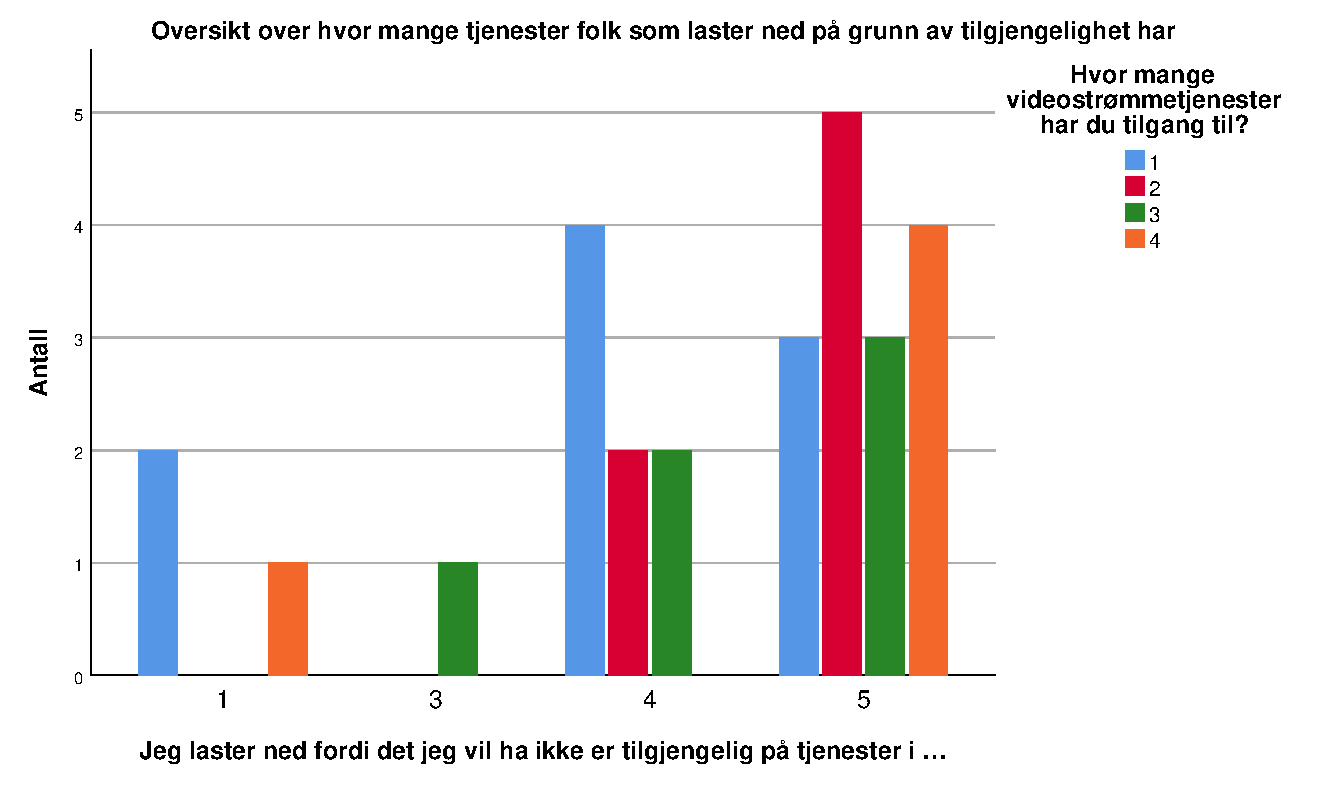
\includegraphics[scale=0.45]{case_1/bilder/tilgjengelighet_antallstromming.pdf}
    \label{fig:tilgjengelighet_antallstromming}
    \caption[Tilgjengelighet vs antall strømmetjenester]{Korrelasjonen mellom de som laster ned på grunn av tilgjengelighet og hvor mange tjenester de har tilgang på}
\end{figure}

Her viser det seg at de som laster ned på grunn av tilgjengelighet også har en god del strømmetjenester. Dette sier at mange av disse er storforbrukere av film og serier, og at det ikke har så mye å si om de har tilgang til tjenestene eller ikke. Dette vil muligens utelukke en løsning i form av at NTNU tilbyr en tjeneste siden de kommer til å laste ned uansett.

\subsection{Konklusjon av verktøy}
Histogrammer er et velkjent og godt verktøy innen statistikk og fungerer godt i mange forskjellige felt, inkludert rotårsaksanalyse.  Det fungerte også veldig bra i denne sammenhengen for å visualisere problemer knyttet til informasjonssikkerhet, og lettere forstå dataene. Siden dataene ble lettere å forstå førte det også til at vi hadde mulighet til å lage flere histogrammer for å analysere mange aspekter ved spørreundersøkelsen. Det negative med histogrammer er hvis de ulike dataene har stor forskjell på antall respondenter i de ulike kategoriene. Da kan det være vanskelig å se sammenhenger og korrelasjoner visuelt sett. Dette kan løses ved å ta et tilfeldig utvalg fra hver kategori og gruppere det opp mot det spørsmålet man ønsker å analysere det med. Da vil det være lettere å se korrelasjoner, men siden vi hadde for lite utvalg kunne vi ikke gjøre dette på alle dataene vi ønsket. Det er likevel enkelt å se korrelasjoner dersom det er signifikante forskjeller eller likheter.

%------------------------------------------------------ANOVA_ANALYSE----------------------------------------------------
\section{Statistisk analyse}
I denne delen benytter vi et par statistiske verktøy for å analysere dataene. Verktøyene vi har brukt er en independent-samples t-test og en one-way ANOVA. Begge disse ble beregnet i det statistiske verktøyet SPSS. Vi regner med en signifikans på \[\alpha \le 0,05\]


\subsection{Ønsket utbytte}
Vi ønsket å benytte en independent t-test for å undersøke forskjeller mellom variabler der den uavhengige variabelen bestod av to grupper. Vi ville utforske om det var noen signifikant forskjell når det kom til om folk laster ned, mellom Kallerud og de andre studentbyene. I tillegg ville vi se på om det var noen signifikante forskjeller mellom IT fakultetet og de andre fakultetene. Ønsket utbytte ved bruk av ANOVA-analysen er å gi oss et bilde av om påstandene har noen signifikant verdi knyttet til demografien.


\subsection{Independent-samples t-test}
Vi valgte å kjøre en independent-samples t-test for å undersøke om det at Kallerud har ti ganger så raskt nett har noen innvirkning på om en laster ned eller ikke. Vi delte opp Kallerud og de andre studentbyene hver for seg, og oversatte nei og ja svarene fra om du hadde lastet ned til henholdsvis 1 og 2. Under ser vi litt statistikk for svarene. 
\begin{figure}[H]
    \centering
    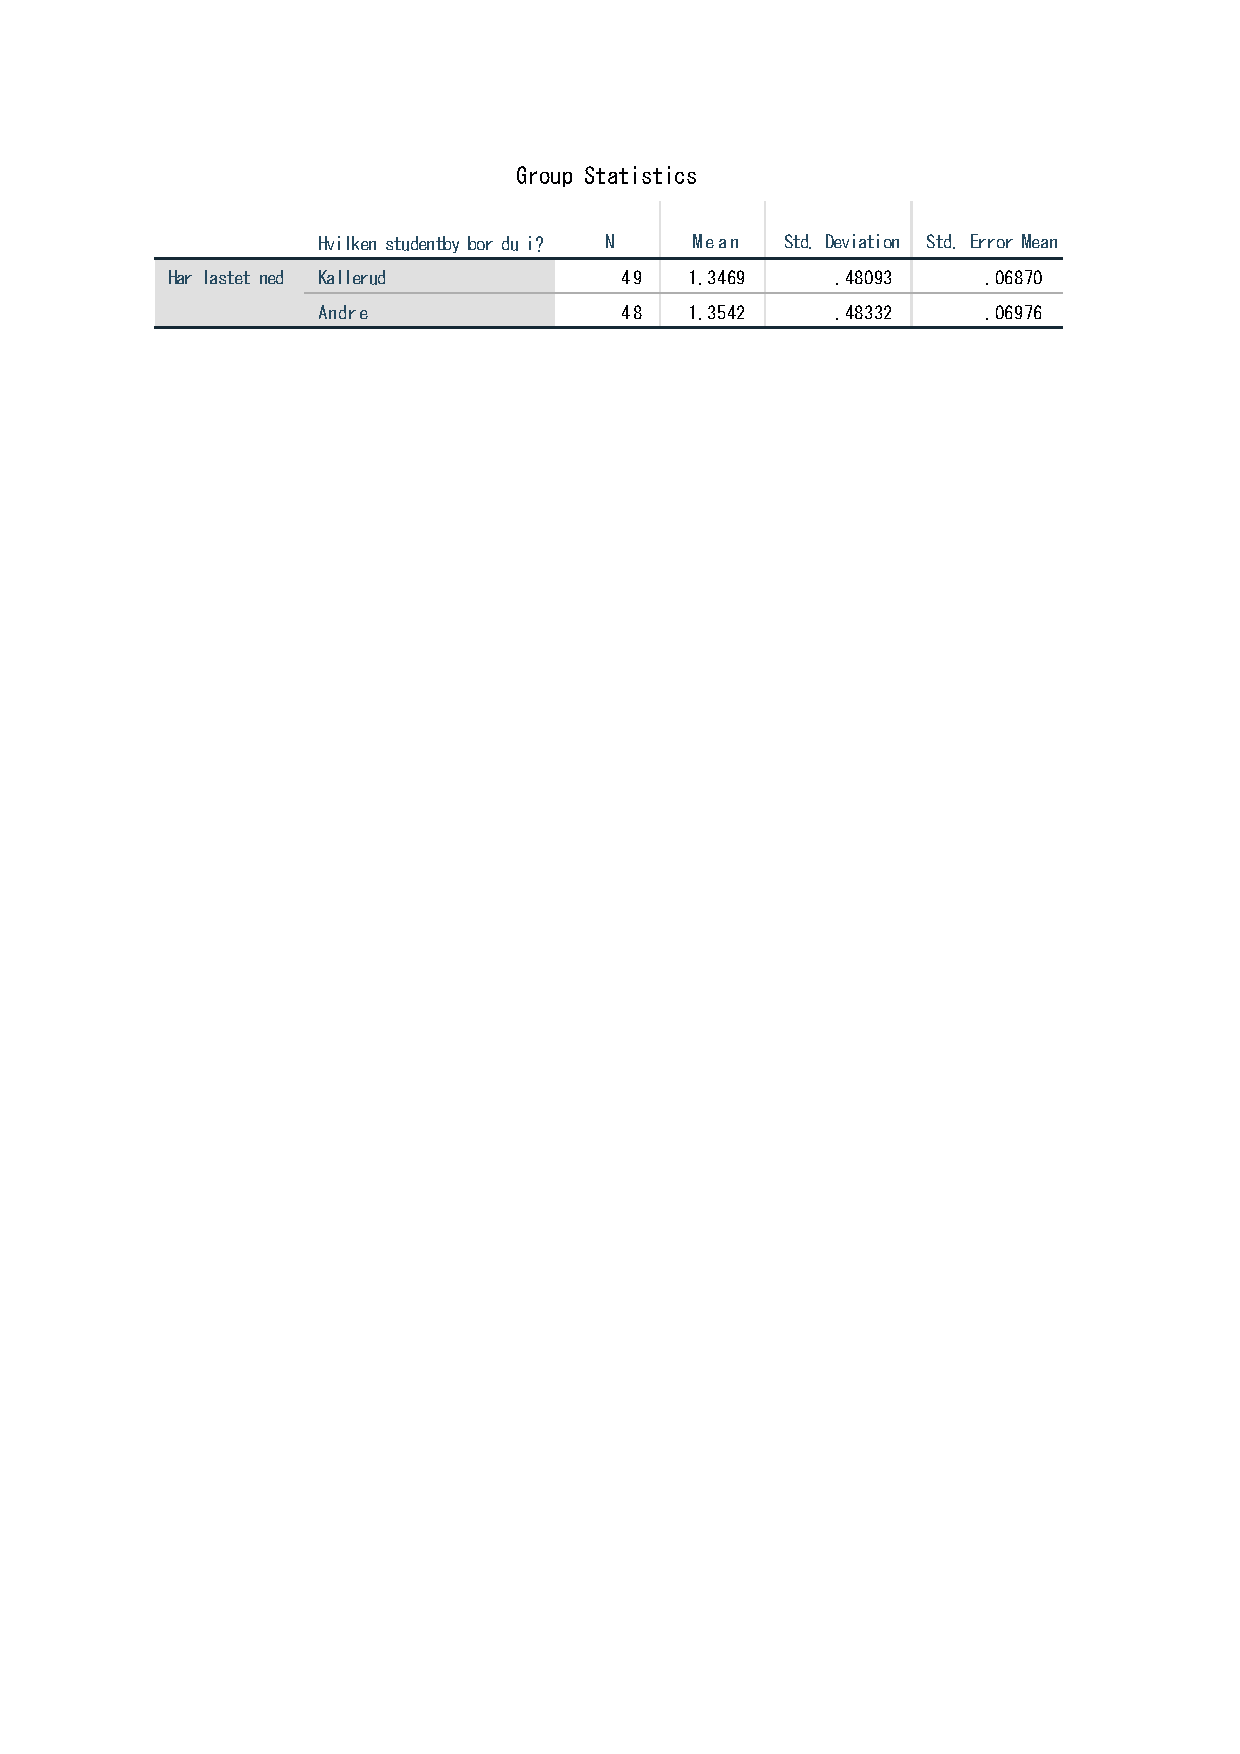
\includegraphics[scale=0.7]{case_1/bilder/studentby_lasterned_ttest_stats.pdf}
    \caption{Gruppestatistikk av studentbyer for om de laster ned eller ikke}
    \label{fig:studby_lasterned_ttest_stats}
\end{figure}

Vi kan allerede her se at svarene ikke differensierer noe særlig. I testen under ser vi selfølgelig derfor at det ikke er noen signifikans.

\begin{figure}[H]
    \centering
    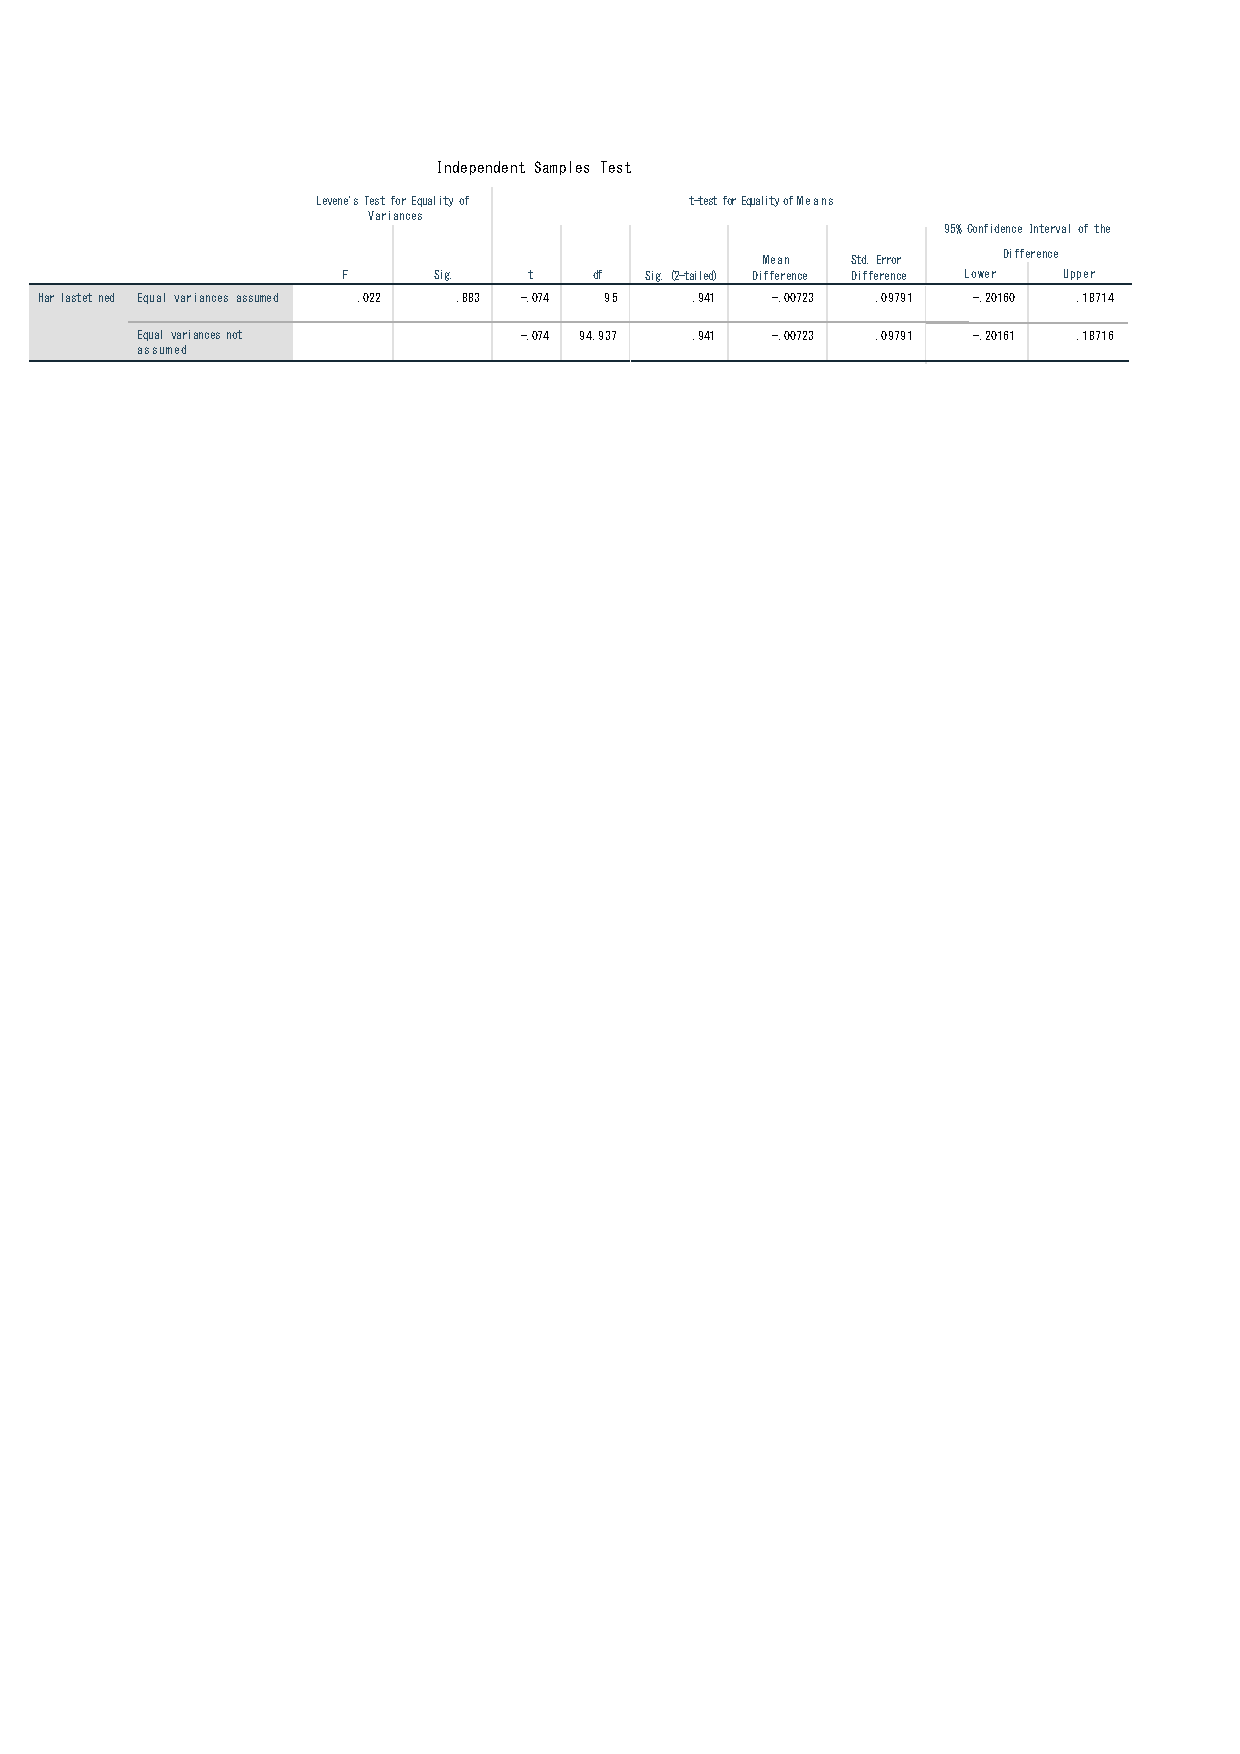
\includegraphics[scale=0.7]{case_1/bilder/studentby_lasterned_ttest.pdf}
    \caption{Independent Samples Test av studentbyer opp mot om de laster ned eller ikke}
    \label{fig:studby_lasterned_ttest}
\end{figure}

Dette betyr at det er ingen forskjeller på personer som bor på Kallerud og de som bor på andre studentbyer når det kommer til om de laster ned, til tross for ti ganger så rask nedlasting og opplasting. 

\subsection{ANOVA-analyse}
I denne analysen ser vi på forskjeller mellom IT fakultetet og de andre fakultetene i henhold til svarene som ble gitt på påstandene. Det ble i tillegg også kjørt analyser basert på kjønn og alder, men med alder var datafordelingen for lav på enkelte alternativer til å kunne si noe om det så den har uteblitt i rapporten. På kjønn brukte vi ANOVA til å se forskjeller i svar på påstandene og kjennskap til IT reglement. Bare kjennskap til IT reglement vises her siden det var det eneste med både tilstrekkelig svar fra hvert kjønn og signifikans i forskjellen.

%-----------------------------------------------ONEWAY ANOVA - fakultet MOT PÅSTAND------------------------
%-----------------------------------------------DESCRIPTIVES------------------------------------------------
\begin{figure}[H]
    \centering
    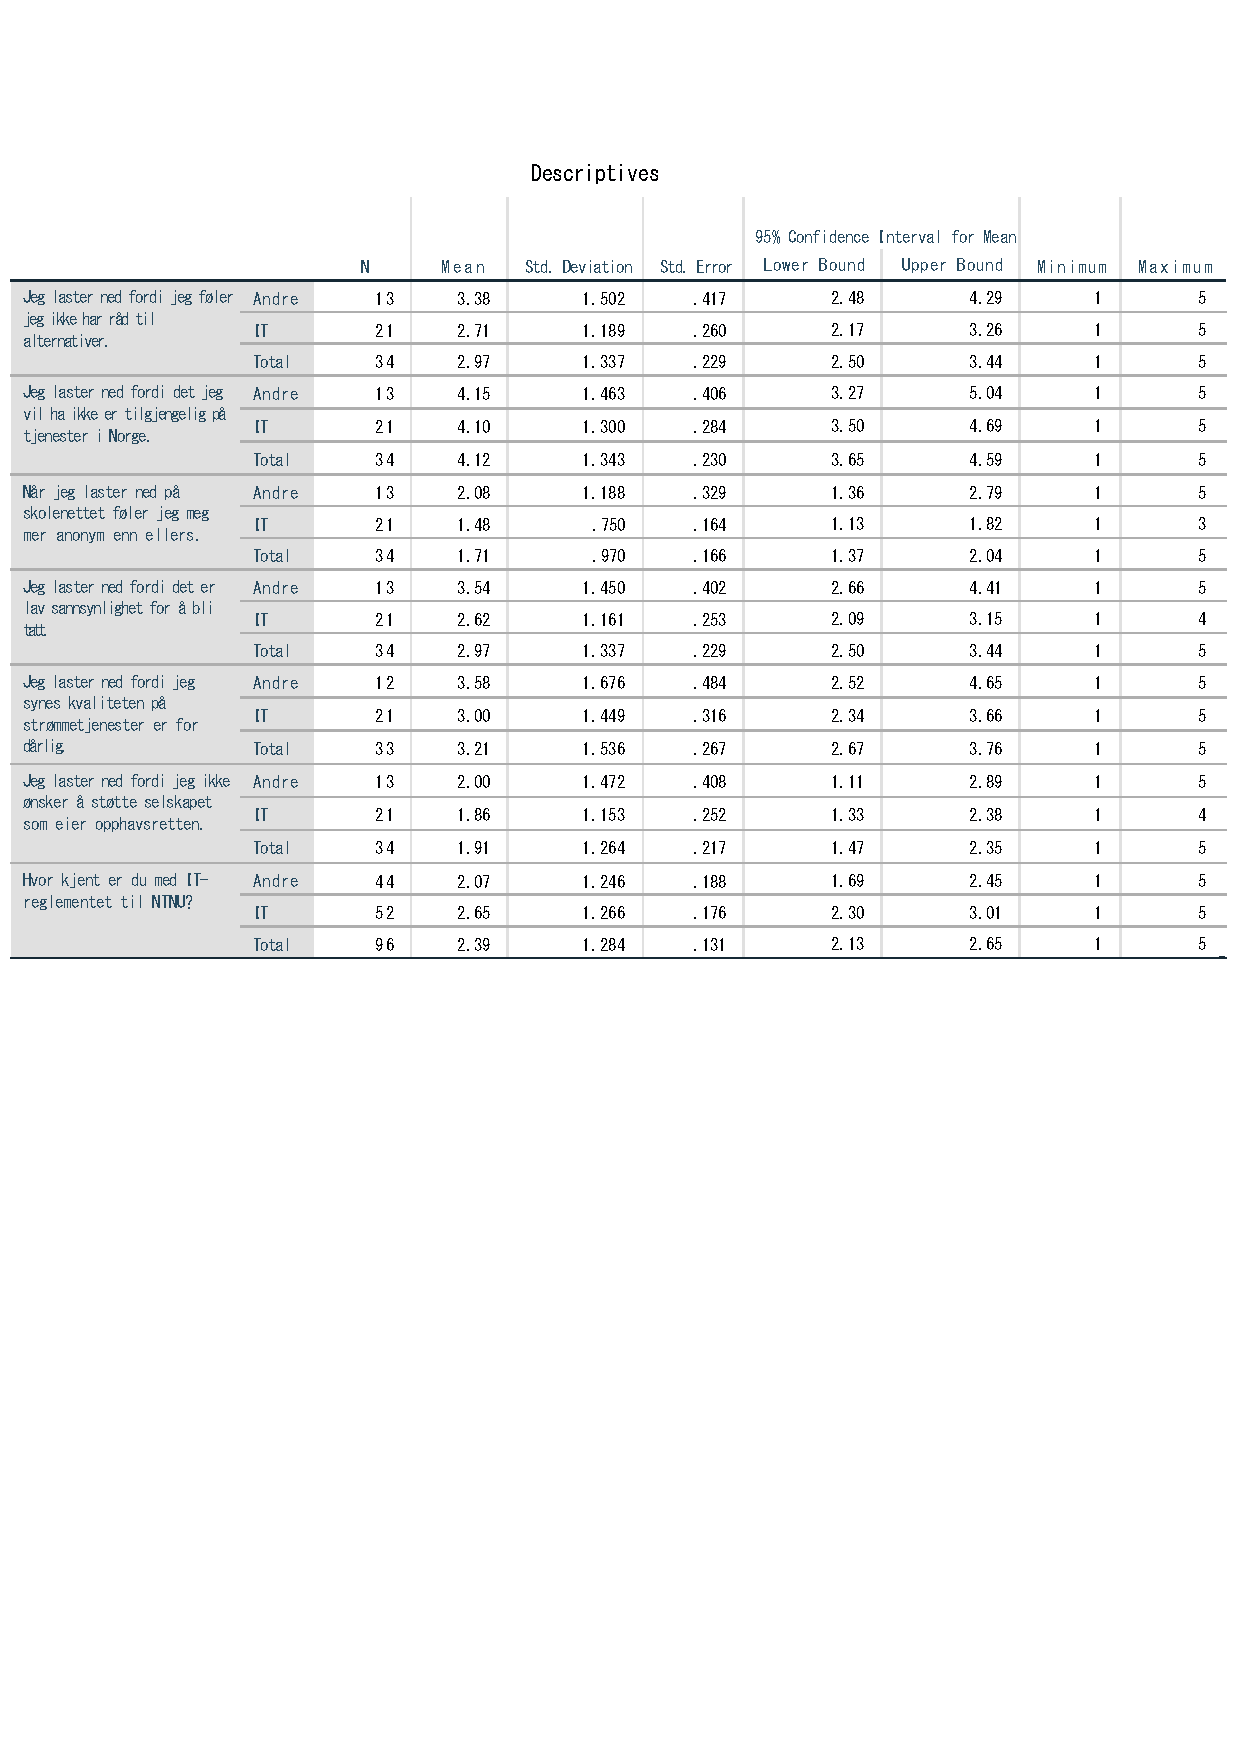
\includegraphics[scale=0.6]{case_1/bilder/fakultet_pastander_descriptive.pdf}
    \caption{Descriptives for IT fakultetet og de andre fakultetene når det kommer til påstander}
    \label{fig:fakultet_pastander_descriptive}
\end{figure}

I tabellen over ser vi at IT studentene sier seg mer uenig i samtlige påstander, noen mer enn andre, mens de er bedre kjent med IT reglementet. Det er spesielt påstandene om råd til alternativer, anonymitet, sannsynlighet for å bli tatt og kjennskap til IT reglementet som er mest relevant å se på. ANOVA analysen under viser om det er noe signifikans mellom svarene. 
%-----------------------------------------------ANOVA-------------------------------------------------------
\begin{figure}[H]
    \centering
    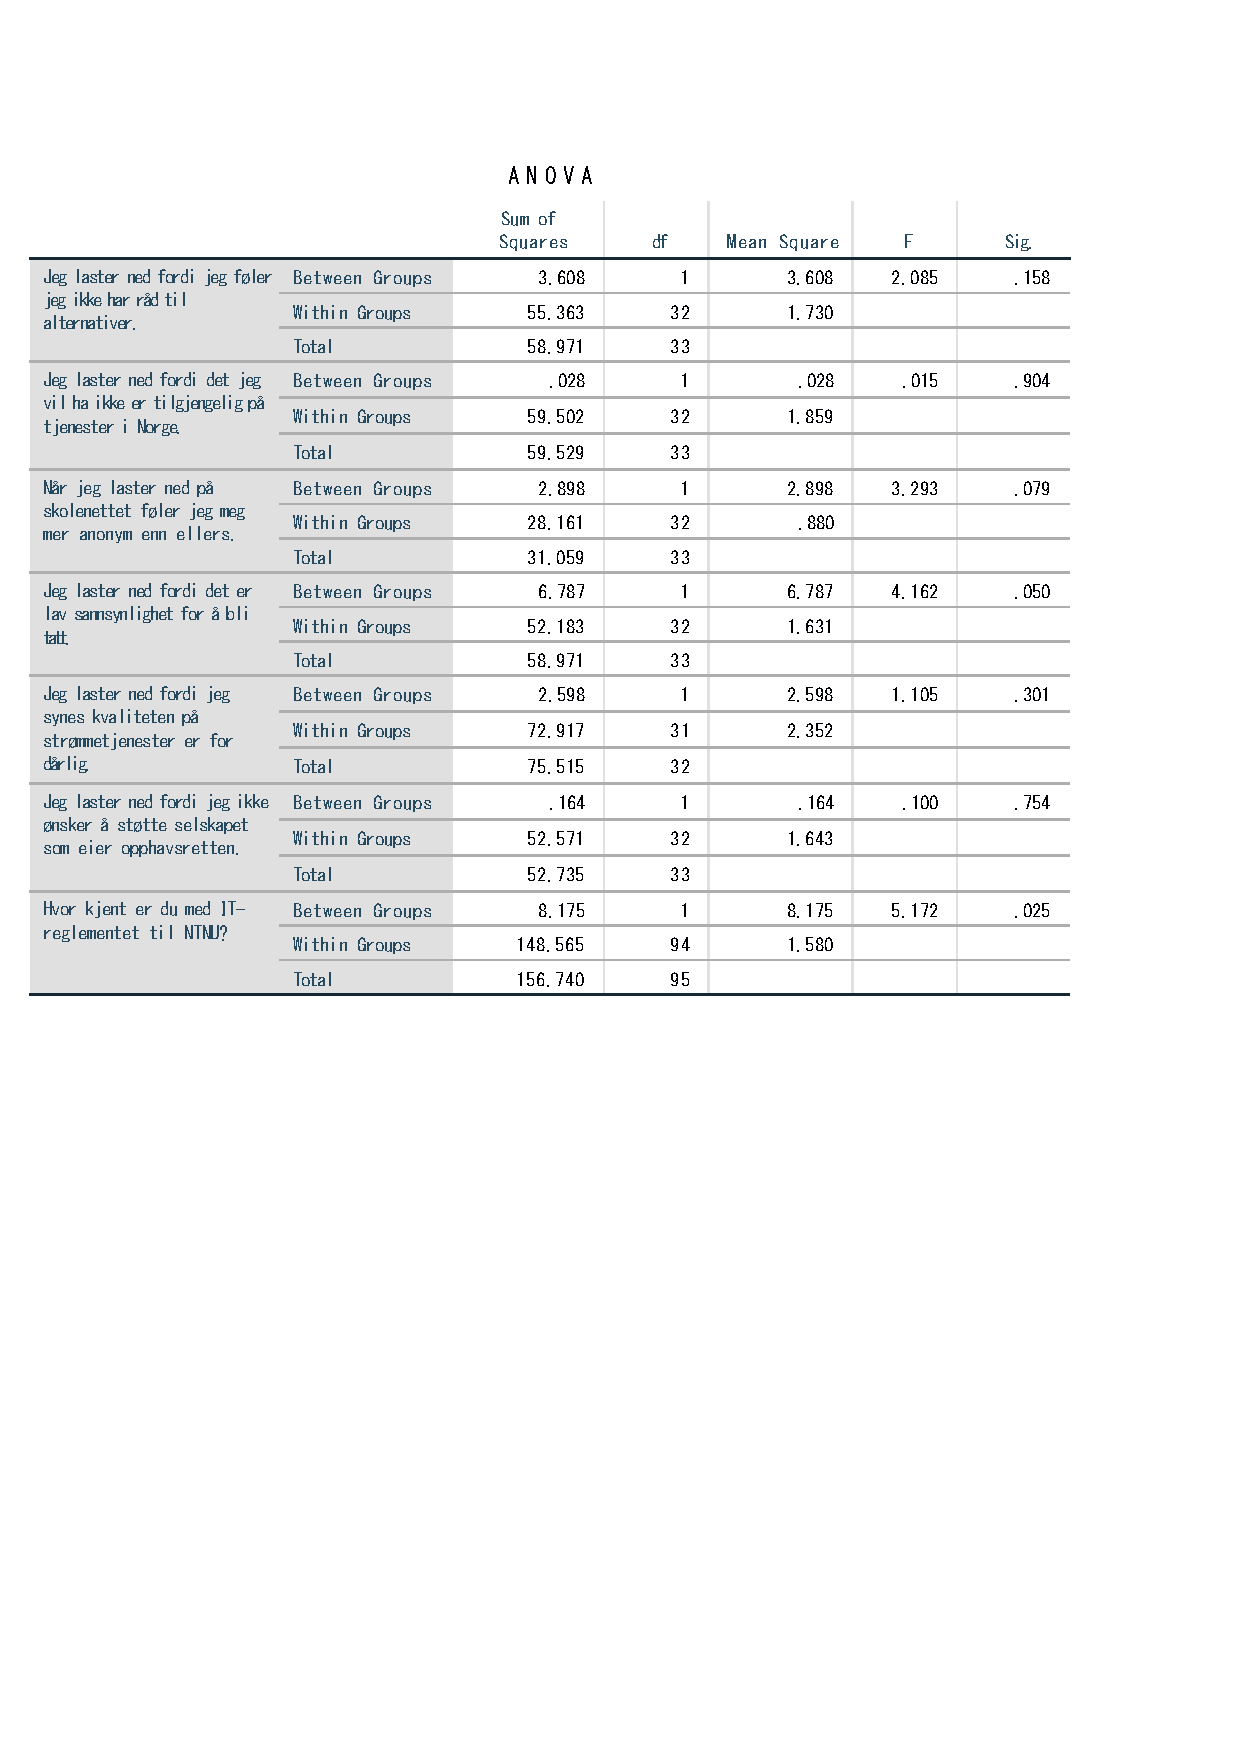
\includegraphics[scale=0.7]{case_1/bilder/fakultet_pastander_anova.pdf}
    \caption{Forskjellen mellom IT fakultetet og de andre fakultetene når det kommer til påstander}
    \label{fig:fakultet_pastander_anova}
\end{figure}

Det viser seg å være signifikant forskjell på IT og de andre fakultetene når det kommer til lav sannsynlighet for å bli tatt og kjennskap til IT reglement. Respondenter fra IT fakultetet er mer uenig i at de laster ned på grunn av lav sannsynlighet for å bli tatt \((\alpha = 0,050)\), og de kjenner også IT reglementet bedre \((\alpha = 0,025)\). 

%-----------------------------------------------DESCRIPTIVES------------------------------------------------
\begin{figure}[H]
    \centering
    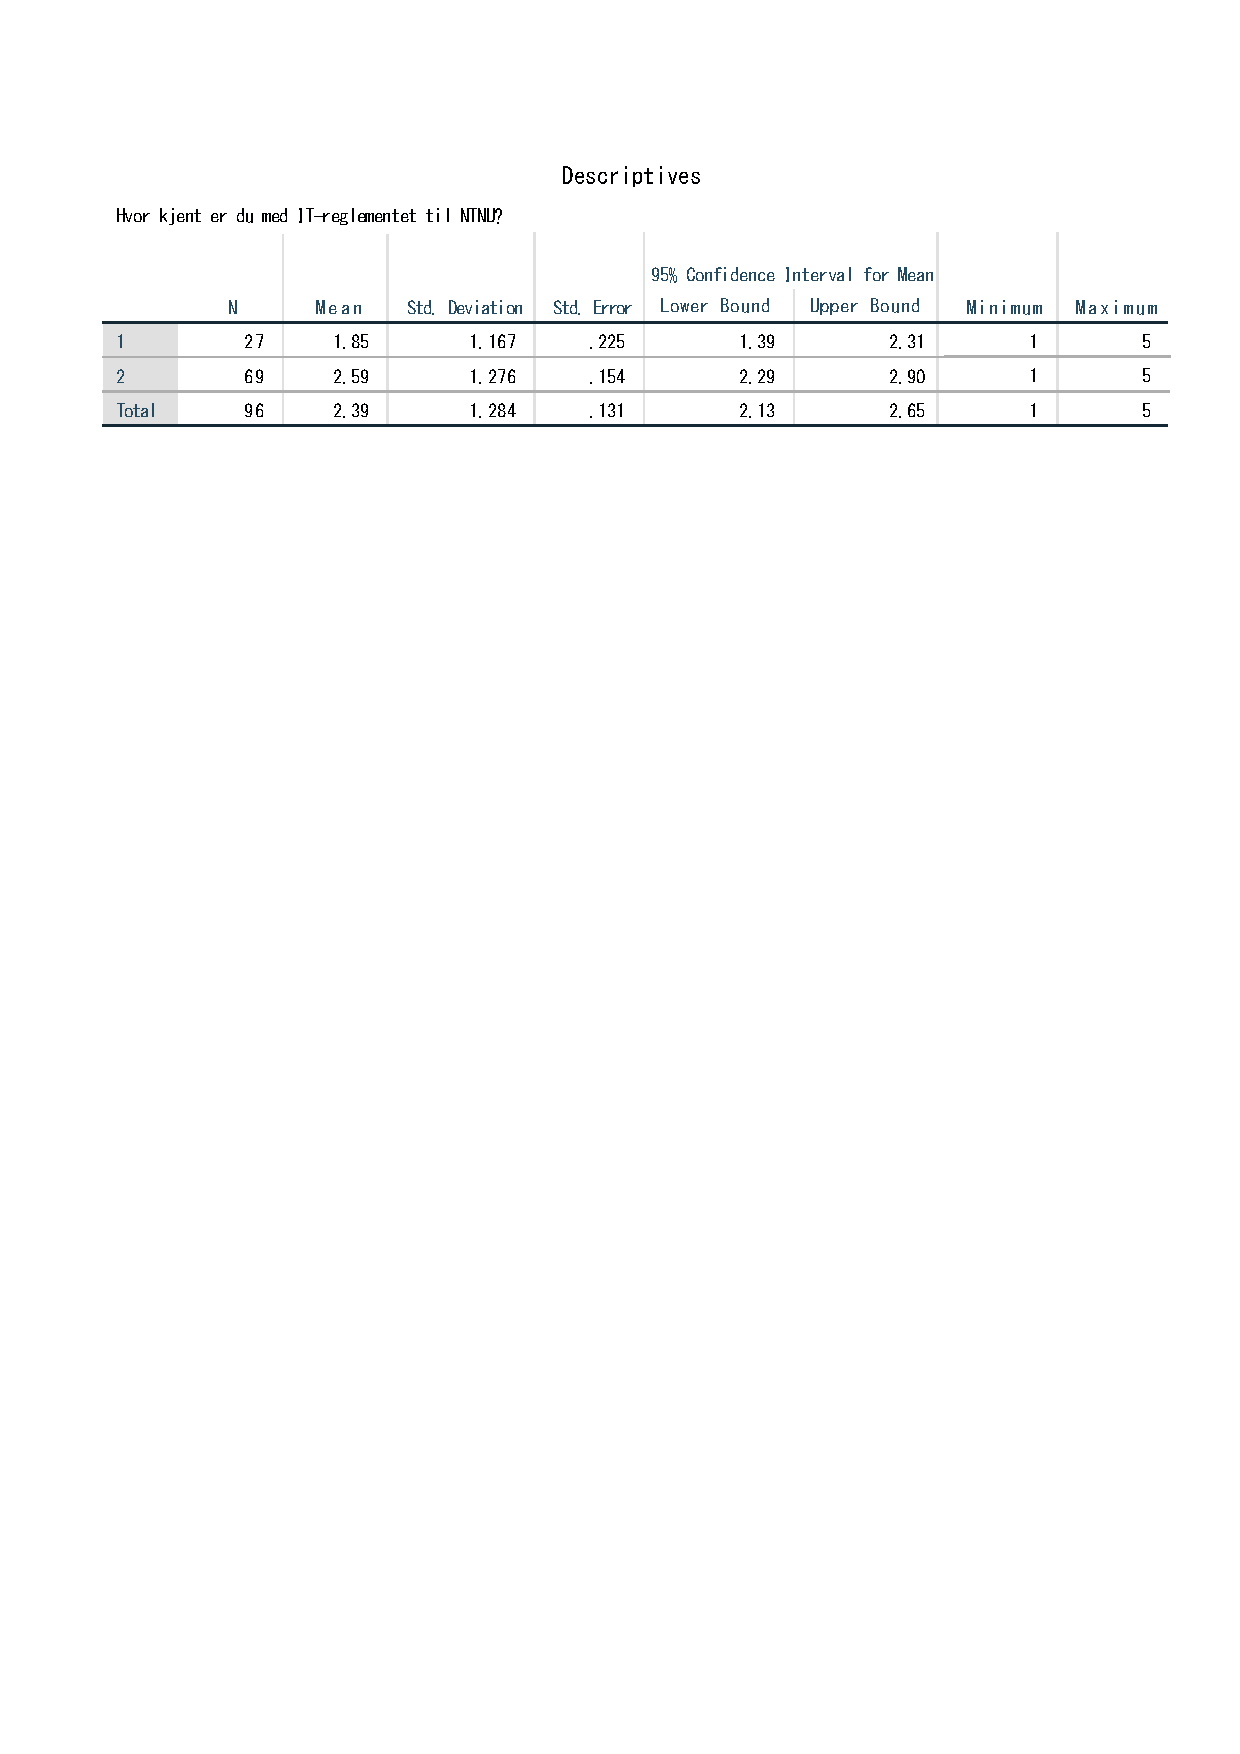
\includegraphics[scale=0.6]{case_1/bilder/kjonn_kjent_descriptive.pdf}
    \caption{Descriptives for kjønn når det kommer til kjennskap til IT reglement}
    \label{fig:fakultet_pastander_descriptive}
\end{figure}

Kvinner er 1 og menn er 2 i disse tabellene. Vi ser fra tabellen over at kvinner svarer at de kjenner til IT-reglementet noe dårligere enn menn. 
%-----------------------------------------------ANOVA-------------------------------------------------------
\begin{figure}[H]
    \centering
    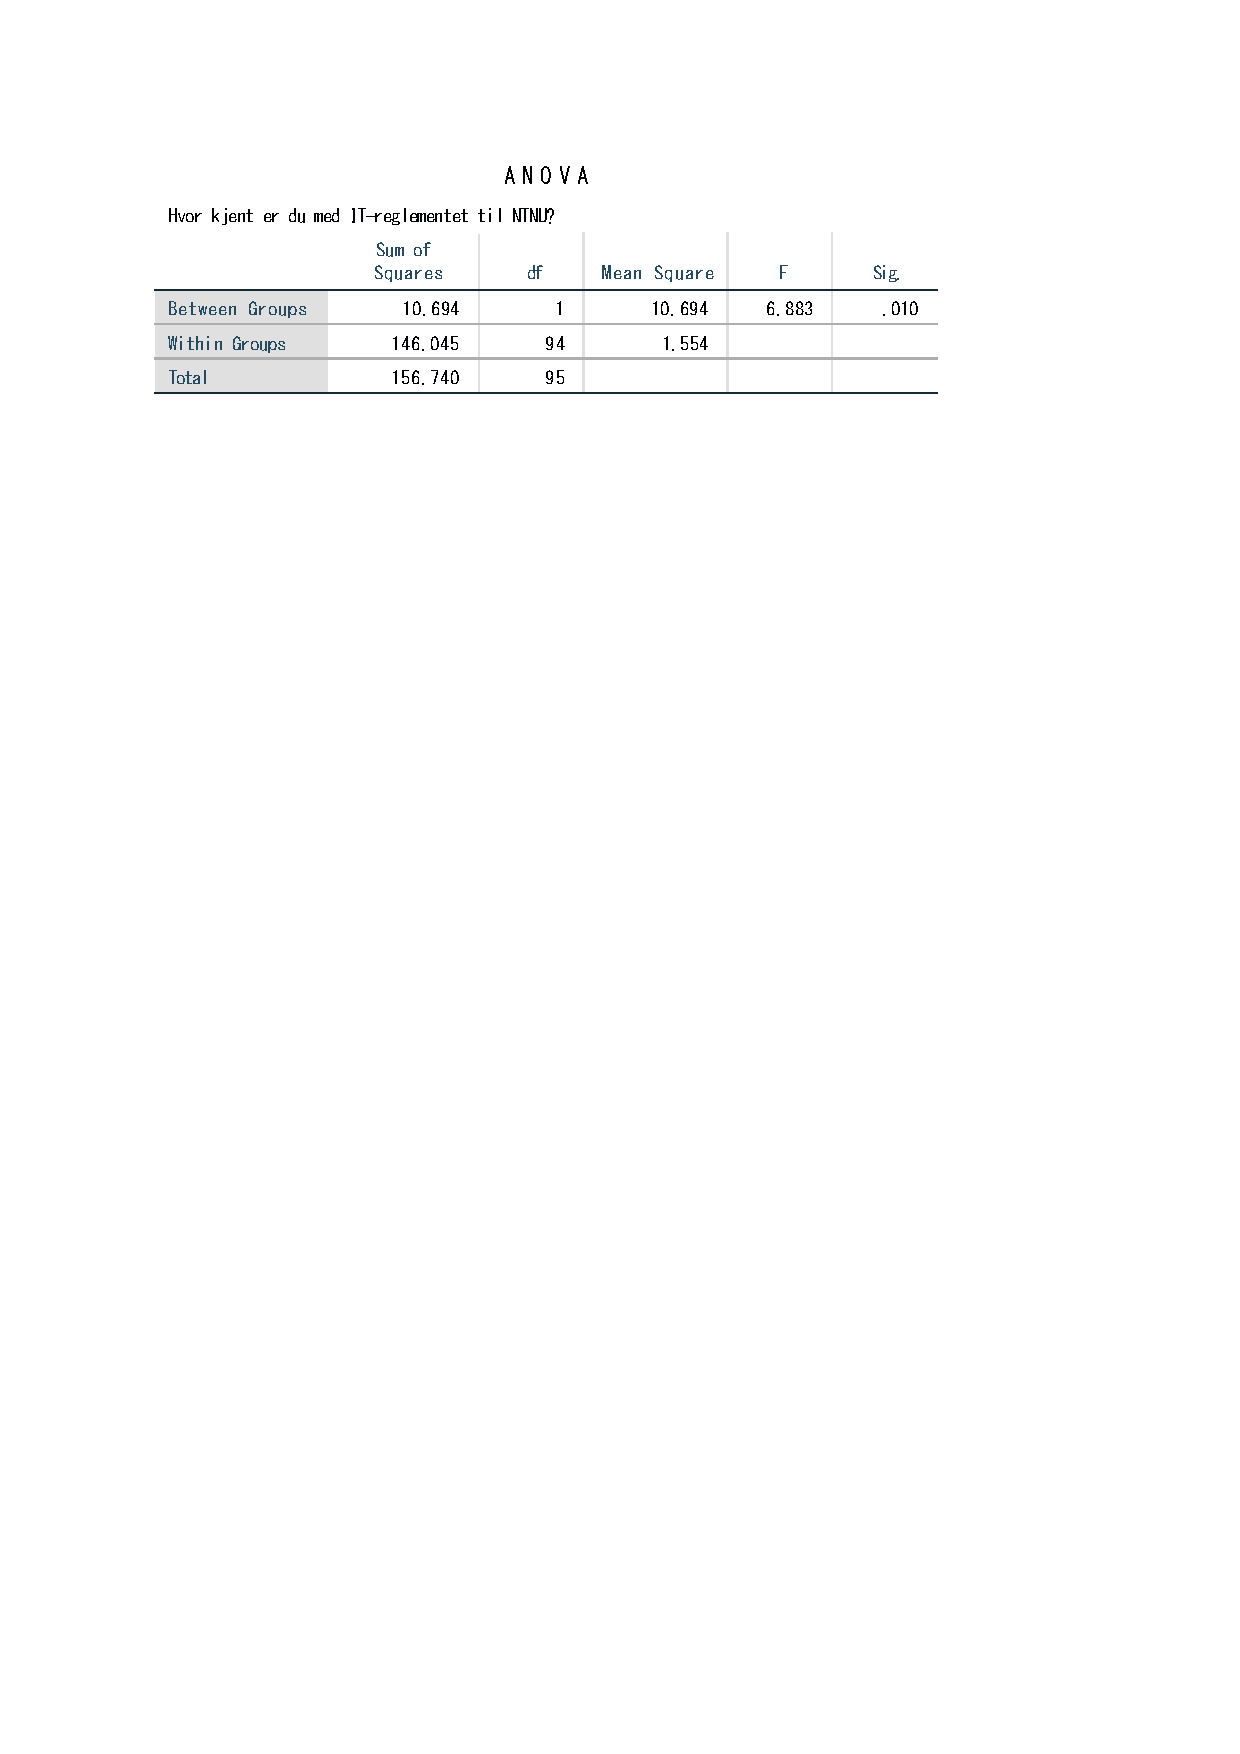
\includegraphics[scale=0.8]{case_1/bilder/kjonn_kjent_anova.pdf}
    \caption{Forskjellen mellom kjønnene når det kommer til kjennskap til IT reglement}
    \label{fig:fakultet_pastander_anova}
\end{figure}

I tabellen over ser vi at menn svarer at de har generelt sett bedre kjennskap til IT reglementet, selv om vi fra tidligere vet at menn er overrepresentert i de som laster ned ulovlig. Noe av det kan forklares med at IT studenter stort sett er menn, og de kjenner reglementet bedre. 

\subsection{Konklusjon av verktøy}
Statistisk analyse var tidkrevende å sette seg inn i for oss som ikke har hatt statistikk fra før. Noe av det var også krevende fordi vi ikke hadde godt nok datagrunnlag til å gjøre alt vi ville. Ellers fungerte det greit til å finne et par signifikante forskjeller i demografien. 

%------------------------------------------------------------------------------------------------------------------------

\section{Affinitetsdiagram}
Affinitetsdiagram brukes til å analysere data som det ikke er mulig å nummerere, eksempelvis meninger eller ideer. Affinitetsdiagram grupperer data og finner de underliggende korrelasjoner og likhetstrekk i gruppen. 

\subsection{Ønsket utbytte}
Ønsket utbytte av affinitetsdiagramet er å få en oversikt over hva deltakerne mener skal til for at de vil stoppe med fildeling.
\subsection{Gjennomføring og resultater}
I spørreundersøkelsen spurte vi om hva som skal til for at deltagerne vil slutte med fildeling. Svarende vi fikk ble sortert inn i 16 grupper organisert under fire hovedkategorier. Hvis noen av deltakere har kommet med flere forslag har hvert av forslagene fått en stemme.  

\begin{figure}[H]
    \centering
    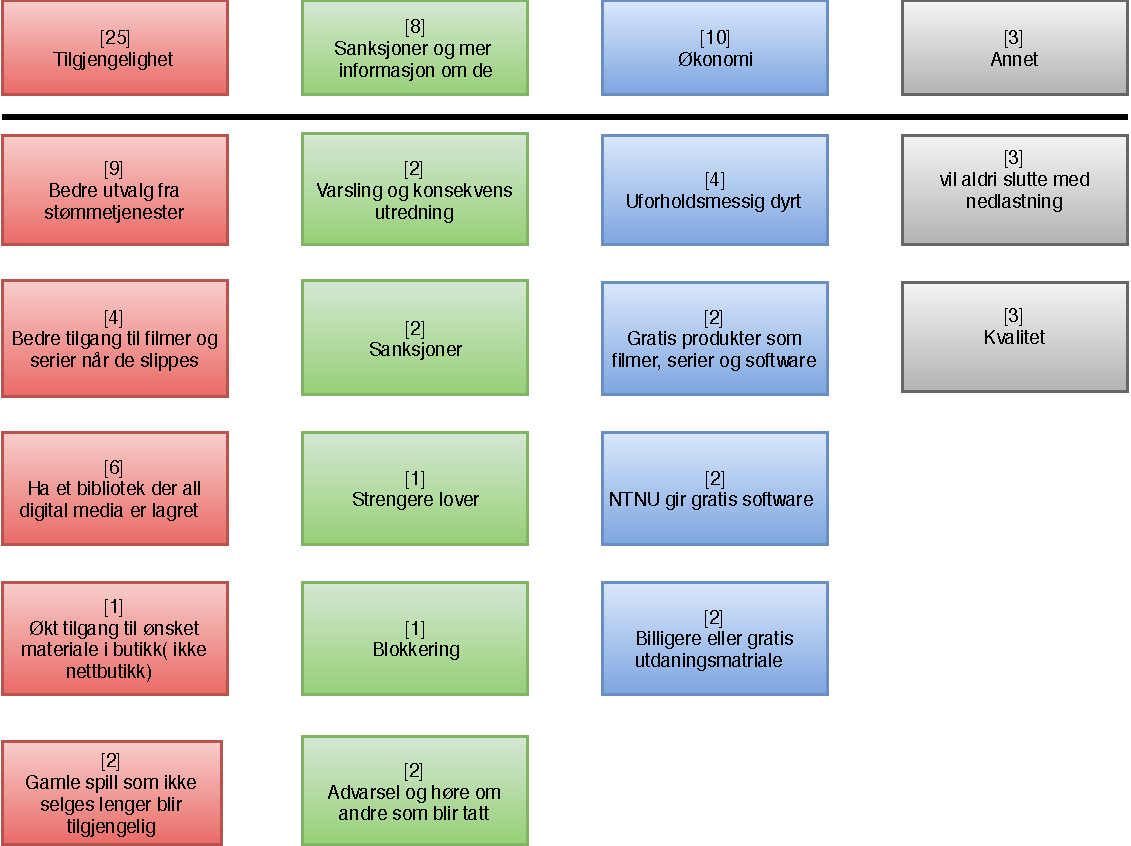
\includegraphics[scale=0.6]{case_1/bilder/stoppe_nedlastning.pdf}
    \label{fig:stoppe_nedlastning}
    \caption{Hva skal til for at personer vil slutte med nedlasting?}
\end{figure}

Denne analysen gir oss ikke rotårsaken til at studenter laster ned, men kan brukes til å gi pekepinne på hva studenter mener skal til for at de vil slutte med nedlasting. Vi kan se på affinitetsdiagram at det er virker å være tre grunner til at personer laster ned. Der det å gjøre materiale mer tilgjengelig virker som den beste løsningen for å stoppe personer fra å nedlaste. Dette samsvarer med de tidligere funnene i figur \hyperref[fig:tilgjengelighet]{Tilgjengelighet}. Problemet med tilgjengelighet er at det er et mer global problem, basert på at en del av de tradisjonell media bruker forsatt geografiske begrensinger. Så da har vi igjen kategoriene økonomi og sanksjoner. Ser man på saksjoner så er det flere som mener at det å være mer vokal om konsekvenser og andre som blir tatt kan være et godt tiltak, som er tildels motstridende med tidligere figur om \hyperref[fig:konsekvens_lasterned]{Konsekvens av å laste ned}. På økonomi eksisterer det et flertall som mener at de har ikke har noe imot å betale for produktet så lenge de mener det er rimelig. Og et mindretall som vil ha gratis produkter. Her kan NTNU kanskje gjøre noe i form av muligens studentrabatter eller de betaler for produktet.          


\subsection{Konklusjon av verktøy}
Affinitetsdiagram er et vektøy som ikke har sin rot i matematikk eller statistikk, men er heller et mer kreativ verktøy der brukerne bruker sin egen tankegang til å finne de korrelerende gruppene. Dette fungerer bra når dataene man henter er på to forskjellige språk og der deltakerne varierer hvor mye de skriver. Siden dataene er blitt organisert inn i grupper er det mye lettere å analysere hva personene mener er viktig. Det negative med affinitetsdiagram er risikoen for at forslag blir gruppert feil eller at det gjøres en feil korrelasjon.        
  

\section{Konklusjon av dataanalysen}
Her diskuteres de funnene som er blitt gjort etter å ha analysert dataene fra spørreundersøkelsen. 

\subsection{Omfang}
Det var 35\% som svarte de hadde lastet ned opphavsrettsbeskyttet materiale i hybelen før, mens 65\% ikke hadde gjort det. Dette var noe lavere enn vi hadde trodd, men omfanget er fortsatt stort og svært problematisk fra skolen sin side. Vi har også sett at de fleste laster ikke ned så veldig ofte. I løpet av en måned laster de fleste ned bare en til tre torrents, eller ingenting i det hele tatt. Allikevel er det i tillegg en god del folk som laster ned over ti torrents i løpet av en måned. Dette vil si at enten så er du en småforbruker eller en storforbruker, det er veldig få i midten, men det er flest av småforbrukerne som vist i figur \ref{fig:antalltorrents}.

\subsection{Demografiske forskjeller og særtrekk}
Gjennom analysen fant vi en rekke forskjeller og særtrekk for de demografiske kategoriene. Det er altså snakk om særtrekk og forskjeller mellom kjønn, fakultet, alder og studentby som er relevant. Alder ble ikke sett så mye på siden litt over 74\% av de spurte var mellom 20 og 25, og vi hadde ikke nok data på de andre som vist i tabell \ref{tab:alder}. 

\subsubsection{Kjønn}
Av de 97 respondentene var det 70 menn og 27 kvinner, altså henholdsvis 72,2\% og 27,8\%. Mellom kjønnene var det store forskjeller på om de hadde lastet ned ulovlig eller ikke. Hos menn var det nesten dødt løp på de som laster ned og de som ikke gjør det, 44.3\% svarte at de hadde lastet ned. Hos kvinner derimot var det bare 11\% som svarte de hadde lastet ned ulovlig på hybelen før. Menn kjenner til IT reglementet noe bedre enn kvinner. 

\subsubsection{Fakultet}
Antall respondenter i de ulike fakultetene var ganske spredt. Det var en sterk overvekt av IT-studenter som svarte på undersøkelsen. Det var 50.5\% av personene som tilhørte Fakultetet for informasjonsteknologi og elektroteknikk. Dette er litt mer enn de andre fakultetene til sammen så vi valgte å ta utgangspunkt i IT fakultetet i forhold til de andre fakultetene siden vi regnet med at det ville være en forskjell der. Og det var det også, studenter tilhørende IT fakultetet har større andel nedlastere enn andre fakulteter. Vi fant også ut at IT studentene hadde bedre kjennskap til IT reglementet enn de andre, selv om de laster ned mer.

\subsubsection{Studentby}
Selv om Kallerud studentby har ti ganger så raskt nett som de andre studentbyene, kan vi ikke vise til noen signifikante resultater som sier det fører til flere som laster ned. Anova-analysen viser at studenter fra Kallerud og de andre studentbyene så og si er likt representert i de som laster ned.

\subsection{Dårlig tilgjengelighet på tjenester}
Dette var hovedfunnet vårt fra histogrammene. Det viste seg at tilgjengelighet på tjenester var en veldig stor grunn til at de fleste valgte å laste ned. Det var bare 4 (11,8\%) som svarte at dette i liten grad betydde noe for dem. Enda færre svarte at de var litt uenig eller nøytral til påstanden, nemlig bare 1 (2,9\%) på hver. Det var derimot 9 (26,5\%) som svarte at de var litt enig, og hele 19 som svarte at de var i stor grad enig med påstanden. Det tilsvarer 55,9\%.
I tillegg til dette ville vi undersøke om de hadde grunnlag til å si dette. Vi laget et histogram som klynget sammen påstanden om tilgjengelighet med hvor mange videostrømmingstjenester de hadde tilgang på. Det var ikke så mange som hadde svart at de var i liten grad enig med påstanden, så datagrunnlaget for å si noe om hvor mange tjenester de som sa seg uenig hadde var vagt.Det viste seg derimot at de som sa seg enig i påstanden også hadde svært mange strømmetjenester, noe som sier at det som er tilgjengelig i Norge ikke er nok til å få dem til å slutte å laste ned. 
I affinitetsdiagrammet var det mange som også så på tilgjengelighet som det store problemet når det kom til hvordan de ville løse det. 25 personer ville stoppet å laste ned hvis det ble gjort noe med tilgjengeligheten. 

\subsection{Alternative tjenester for dyrt i forhold til hva du får}
Respondentene svarer ganske spredt på at de laster ned fordi de føler de ikke har råd til alternativer. I tillegg til det svarer ti stykker i affinitetsdiagrammet at de hadde stoppet å laste ned dersom det ikke var uforholdsmessig dyrt eller hvis noen hadde tilbudt gratis tjenester. Siden det også er mange som ikke bryr seg om økonomien når det kommer til nedlasting er ikke dette funnet like relevant som tilgjengeligheten, men det er verdt å ta i betraktning. Dette var overraskende siden vi hadde trodd dette betydde mye mer for folk enn det egentlig gjør. 

\subsection{Dårlig håndhevelse og kommunikasjon av eksisterende lover}
I undersøkelsen svarte 47.4\% at de ikke kjente til konsekvenser ved brudd på opphavsretten. Det viser seg også at generelt sett de som laster ned kjenner konsekvensene bedre enn de som ikke gjør det. Dette viser at selv om de kjenner til konsekvensene laster de ned uansett fordi sjansen for å bli tatt for det er tilnærmet null. Det var også svært få som kjente til NTNU's IT reglement, som blant annet viser til norske lover angående krenking av opphavsrett og ulovlig fildeling. Sanksjoner for brudd på reglementet kan være utestengelse av nettet i opptil fem dager, men driftsansvarlige er dårlige til å håndheve disse reglene, selv om det er krav om det i reglementet \cite{ITReg}. 